%----------------------------------------------------------------------------------------
%
% LaTeX-template for degree projects at LNU, Department of Computer Science
% Last updated by Johan Hagelbäck, Oct 2015
% Linnaeus University
%
% License: Creative Commons BY
%
%----------------------------------------------------------------------------------------

%----------------------------------------------------------------------------------------
%	Settings and configuration
%----------------------------------------------------------------------------------------

\documentclass[a4paper,12pt]{article}

\usepackage[T1]{fontenc}
\usepackage{times}
\usepackage[english]{babel}
\usepackage[utf8]{inputenc}
\usepackage{url}
\usepackage{array}
\usepackage{wallpaper}
\usepackage[absolute]{textpos}
\usepackage[top=2cm, bottom=2.5cm, left=3cm, right=3cm]{geometry}
\usepackage{appendix}
\usepackage[nottoc]{tocbibind}

\setcounter{secnumdepth}{3}
\setcounter{tocdepth}{3}

\usepackage{sectsty}
\sectionfont{\fontsize{16}{15}\selectfont}
\subsectionfont{\fontsize{14}{12}\selectfont}
\subsubsectionfont{\fontsize{12}{12}\selectfont}

\usepackage{csquotes} % Used to handle citations

\renewcommand{\thetable}{\arabic{section}.\arabic{table}}
\renewcommand{\thefigure}{\arabic{section}.\arabic{figure}}

\newsavebox{\mybox}
\newlength{\mydepth}
\newlength{\myheight}





\begin{document}


\pagenumbering{gobble}
\pagenumbering{arabic}

%----------------------------------------------------------------------------------------
%
%	Here follows the actual text contents of the report.
%
%----------------------------------------------------------------------------------------
	\title  { Assignment Report}
	\maketitle
	\section{Introduction}
This is the first assignment of the course Computer Networks and it is about creating a UDP/TCP socket in java. The codes is to be tested by creating an environment in a virtual networking.

\begin{itemize}
\item The first part is about creating the connection and setting up the virtual network environment.
\item The Second part is to implement the UDP connection
\item The third part is to implement the TCP connection
\item The last part is about capturing the traffic by using the software Wireshark.
\end{itemize}
The report will address the way the problems were solved and the some pictures were add to show the results. 



\section {Problem One :}

This problem was about setting up the virtual machine environment. By following the guidance everything went smooth. One kind of trouble was to set up the Host-only adapter as in the beginning there was no default vboxnet(). The next screenshot I took after finish the set up and calling ping -c 5 of the IP address of the virtual machine from the host machine. We can see in the picture the Time to Live which is 64. Moreover, in the statistics, we can see the minimum round trip, the average and the max.
\begin{figure}[h]
    \centering
    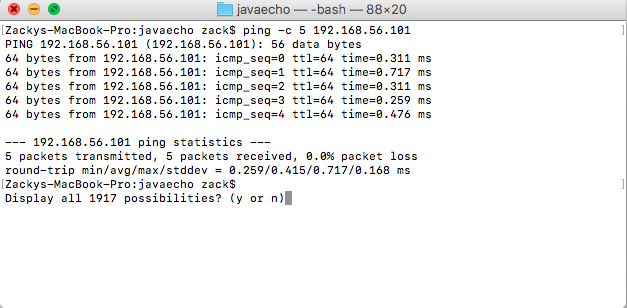
\includegraphics[width=0.65\textwidth]{ping}
    \caption{pinging the IP address of the server from the client machine}
    \label{fig:mesh1}
\end{figure}

\newpage



\section {Problem Two}
This problem was about implementing the configuration of the buffer size and the message rate. 
\begin{figure}[h]
    \centering
    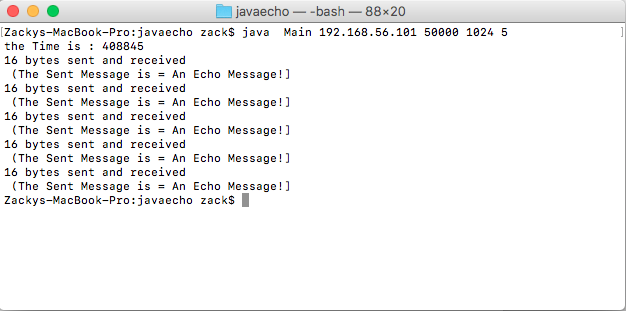
\includegraphics[width=0.75\textwidth]{figure2}
    \caption{Sending messages from client to server by UDP}
    \label{fig:figure2}
\end{figure}

As we can see in the figure 3.2, By running the main class in terminal and providing the IP of the server machine and the transfer rate which is the desired number of messages per seconds and the port address. In the next example I tried 5 messages per second. By using a thread, I tended to stop the simulation after 1 second as it is asked in the first VG task to make the mechanism works properly. In case the transfer rate is so high the client will send as many messages as it can in 1 second and print the number of the sent messages and the 
number of the ones that were not able to be send (as you can see in figure 3.3). 
\begin{figure}[h]
    \centering
    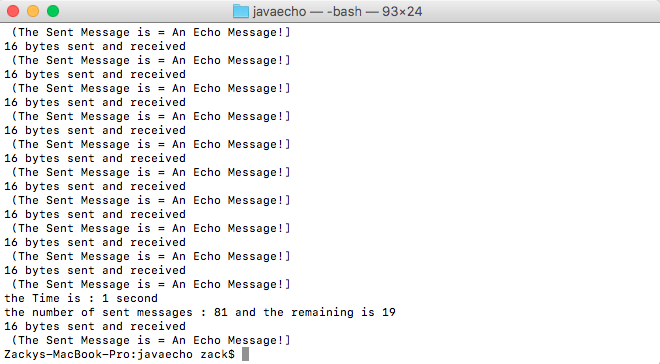
\includegraphics[width=0.75\textwidth]{figure3}
    \caption{The transfer rate is 100. After 1 sec it notifies user how many messages were sent}
    \label{}
\end{figure}



Finally an abstract class networkLayering was implemented for the VG-task 2 with some methods that are being used in UDPEchoClient class and are going to be used in TCPEchoClient. 
In the abstract there is Run method as the abstract implements Runnable class. Moreover, some other methods such as RunClient, Delay, RunTheThread  and ErrorHandler.



\subsection {Handling the error:}
I implemented an error handling method in the networkLayer class. It gives messages for some error that might occur while the user enters the command to send messages from the client server. 
\begin{itemize}
\item	First a method that checks if the IP is valid or in a right format. That is the IP address should be consisted of 4 parts and the numbers between 0-255.
\item A function that checks if the port number is valid. Since the port number is an unsigned 16-bit integer so it should be in the range (1-65535)
\item	A function to check the transfer rate. The transfer rate should not be less than 1 as if it is zero so no messages will be sent and it cannot defiantly be less than zero.
\item	In the UDPEchoClient class, there is a function to check the message length. The longest a message can be that does not cause a failure in the program is 65507. That is because the IP header is 20 and the UDP header is 8, thus 65535-20-8 =65507 byte. The function checks as well if the message is empty and notify the user.
\item	Lastly, there is a function that checks if the number if arguments that entered by the user is right. The program asks the user to give an IP address, Transfer rate and a port number. 

\end{itemize}

\begin{figure}[h]
    \centering
    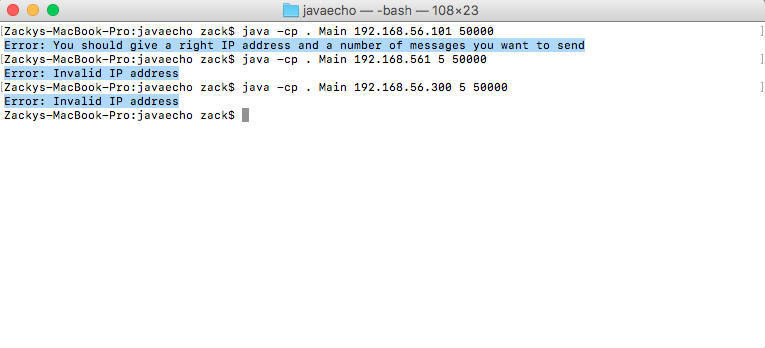
\includegraphics[width=0.75\textwidth]{figure10}
    \caption{Some example of the error messages}
    \label{}
\end{figure}


\newpage
\section{Problem Three: }
This problem was about implementing a TCP connection between the host machine and the virtalbox machine. I used some codes from the previous problem and needed some new ones. However, the TCPEchoClient class is implementing the abstract class networkingLayer for the thread and the error handling. 
In figure 4.5 we can see that I sent a message with a size 100 while the buffer size in the abstract class was set to 64 and the client still sent and received the whole message.

\begin{figure}[h]
    \centering
    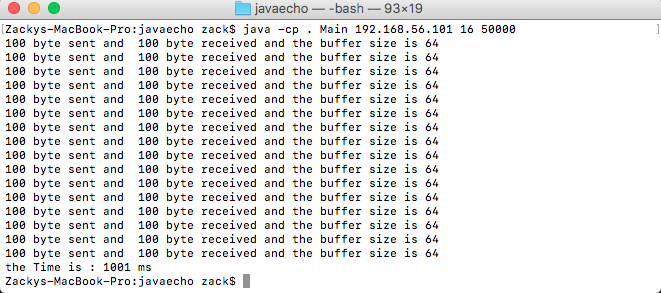
\includegraphics[width=0.75\textwidth]{figure4}
    \caption{In TCP the client received the whole message even if the  buffer size is small
    }
    \label{}
\end{figure}


While in Figure 4.6 and by repeating the same procedure but on the UDP connection we see that 100 bytes were sent but 64 was received which is the size of the buffer. That is explained in the definition of stream-oriented connection. In other words, TCP works on gathering the byte contiguously by streaming them and putting them into one segment or more. That is why TCP keep track of the whole message boundaries and send it all. 


\begin{figure}[h]
    \centering
    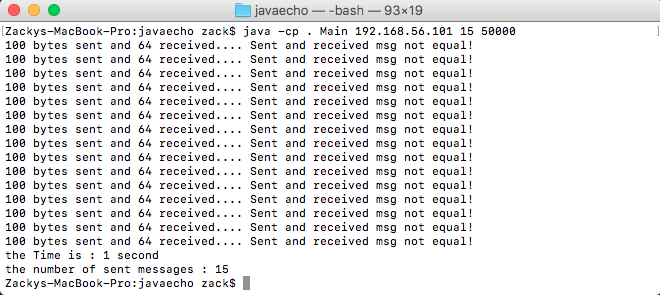
\includegraphics[width=0.70\textwidth, ]{figure5}
    \caption{In UDP the client received the message according to the buffer size}
    \label{}
\end{figure}



\newpage
\section{Problem Four: }
\subsection{UDP trafic capturing}
In this problem I run the same code and captured the traffic by Wireshark. In Figure 5.7 I had small buffer size while in Figure 5.8 I had a buffer size that fit the message length. There was no different in the length as the wireshark shows that the length of the sent and the received message is the same.

\begin{figure}[h]
    \centering
    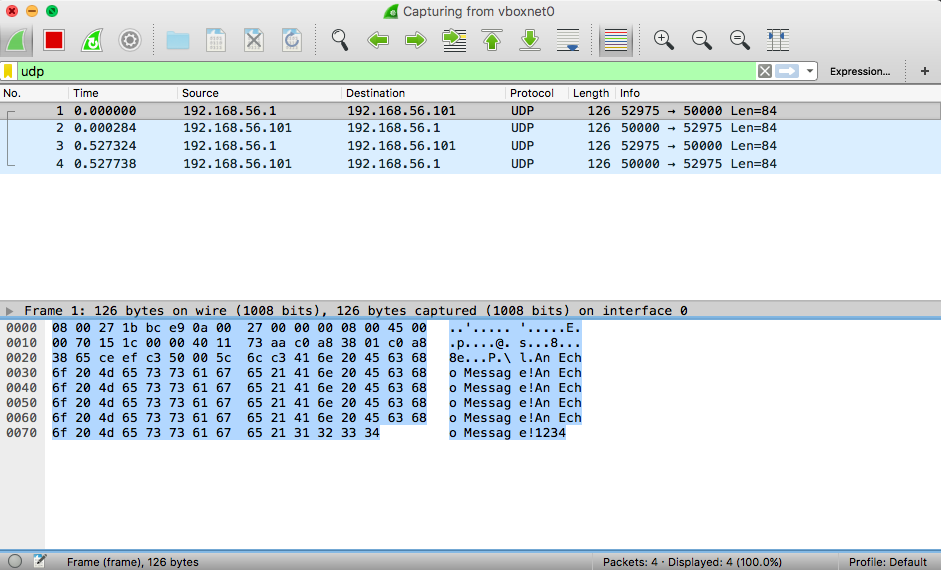
\includegraphics[width=0.70\textwidth]{figure6}
    \caption{The buffer size is set to be enough for the message size}
    \label{}
\end{figure}

\begin{figure}[h]
    \centering
    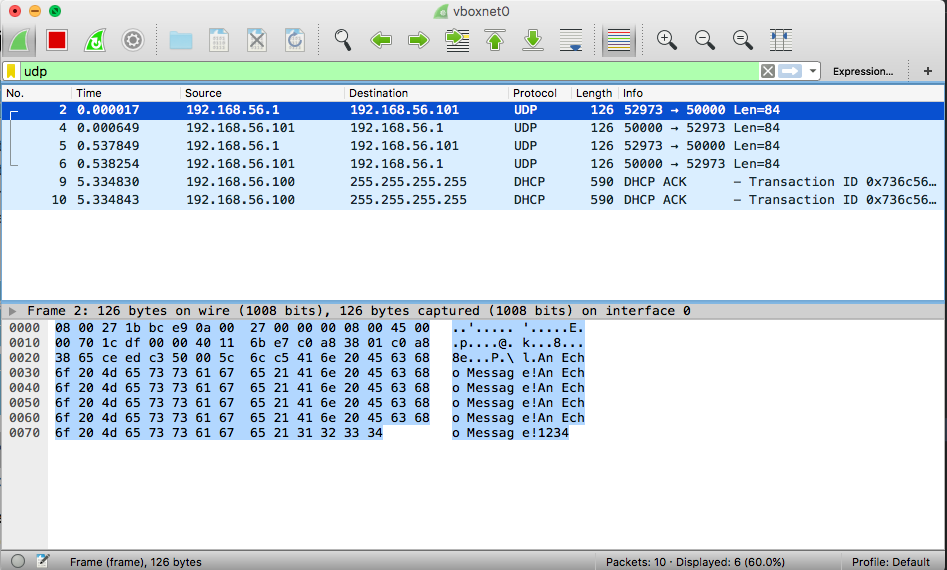
\includegraphics[width=0.75\textwidth]{figure7}
    \caption{The buffer size is set to be smaller than the message size}
    \label{}
\end{figure}

\newpage

\subsection{TCP trafic capturing}
In TCP the server and the client create a connection so even though I am sending the same number of messages which is 2, we see that there is more traffic when it comes for TCP and that is because the three way shake. 
In the first line in Figure 5.9  there is a request from the host machine with sequence number 0 and here the host machine is asking to create a connection by synchronise request.
In the second line, the virtual machine is replying and accepting by sending (SYN - ACK) message. While in third line, the host machine is replying by ACK message and this means that the host machine acknowledges the request and the connection is created.
Then the flag PSH will be set to start sending the messages.	In the TCP there is as well no difference when the buffer size is smaller or bigger than the message size if compare the figure 5.9 and 5.10

\begin{figure}[h]
    \centering
    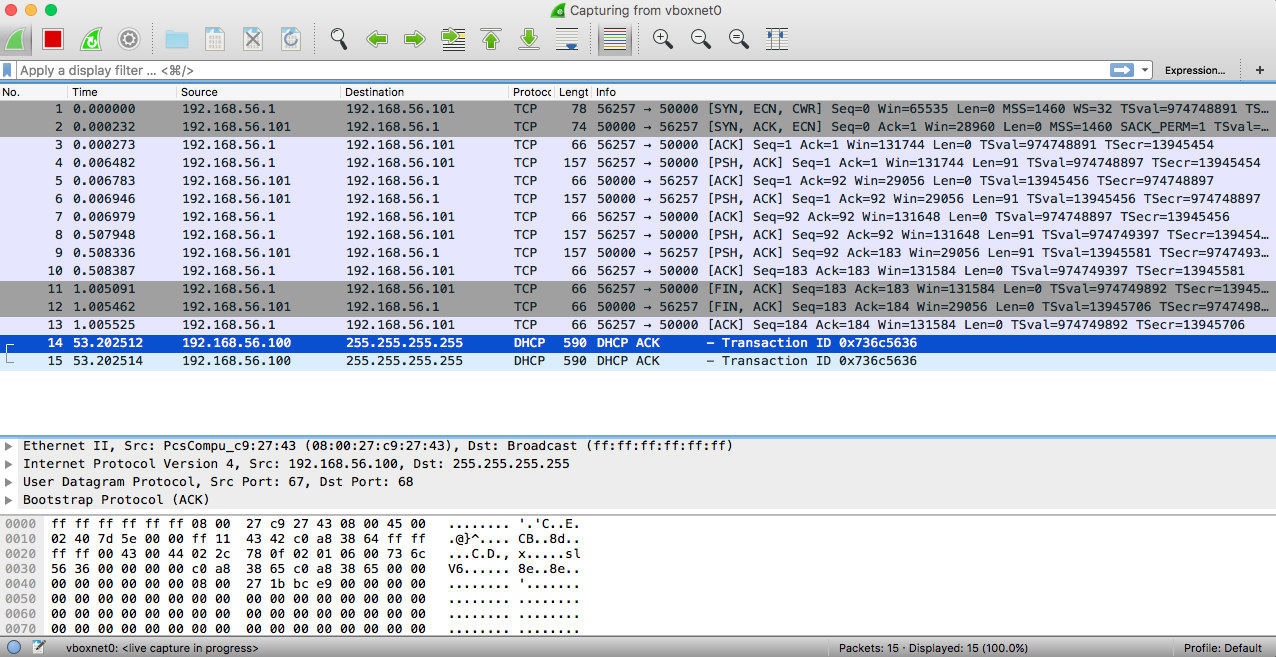
\includegraphics[width=0.75\textwidth]{figure8}
    \caption{The buffer size is set to be enough for the message size}
    \label{}
\end{figure}

\begin{figure}[h]
    \centering
    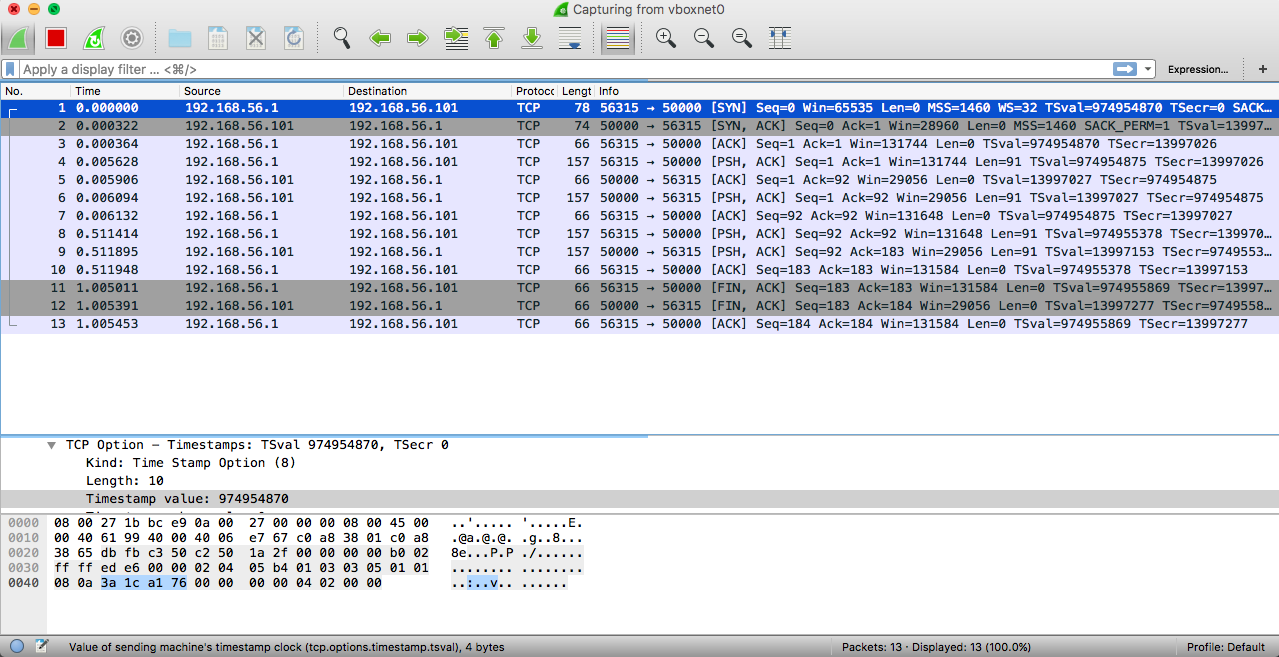
\includegraphics[width=0.75\textwidth]{figure9}
    \caption{The buffer size is set to be smaller than the message size}
    \label{}
\end{figure}


Finally, and as a conclusion of the experiment, we can see that the UDP is connectionless while the TCP use connection to transmit messages. 
TCP is slower and that is because the time establishing the connection take. One more thing to be noticed in the pictures is that the final message size after appending the header is smaller in UDP and that is because the TCP header is 20 bytes while the UDP header is 8 bytes.
The way TCP streams bytes make it reliable and here we mean that it guarantees that there will be no lost data while transmitting it. On the other hand, UDP does not guarantee that and not even getting the data in a right order. 



 
\end{document}